\documentclass[12pt]{article}
\usepackage[catalan]{babel}
\usepackage[utf8]{inputenc}
\usepackage{listings}
\usepackage{color}
\usepackage{graphicx}
\usepackage{verbatim}
\usepackage[obeyspaces]{url}
\usepackage{appendix}
\usepackage{dirtytalk}

\definecolor{codegreen}{rgb}{0,0.6,0}
\definecolor{codegray}{rgb}{0.5,0.5,0.5}
\definecolor{codepurple}{rgb}{0.58,0,0.82}
\definecolor{backcolour}{rgb}{0.95,0.95,0.92}
 
\lstset{
	backgroundcolor=\color{backcolour},   
	breaklines=true, 
	numbers=left,
	basicstyle=\footnotesize,
	backgroundcolor=\color{backcolour},   
    commentstyle=\color{codegreen},
    keywordstyle=\color{magenta},
    numberstyle=\tiny\color{codegray},
    stringstyle=\color{codepurple},
    basicstyle=\footnotesize,
    breakatwhitespace=false,         
    breaklines=true,                 
    captionpos=b,                    
    keepspaces=true,                 
    numbers=left,                    
    numbersep=5pt,                  
    showspaces=false,                
    showstringspaces=false,
    showtabs=false,                  
    tabsize=2
}
\setlength{\parindent}{0pt}

\begin{document}
\begin{titlepage}
		\centering
		
\includegraphics[width=0.5\textwidth]{imatges/logo3.png}\par\vspace{1cm}
		{\huge\bfseries Projecte final\par}
		\vspace{1cm}
		{\scshape\Large Màster en enginyeria informàtica\par}
		\vspace{1.5cm}
		{\Large\itshape Oscar Galera i Alfaro\par}
		\vspace{1cm}
		{\Large\itshape Disseny i implementació de xarxes i sistemes distribuïts\par}
		\vspace{2cm}
		\vfill
		\vfill
		{\large \today\par}
\end{titlepage}
\clearpage
\tableofcontents
\clearpage
\listoffigures


\clearpage
\section{Problema\label{problema}}
El problema a resoldre, és l'obtenció del posicionament i tipologia de sensors (respectant un cost màxim) en una xarxa de distribució d'aigua. 
\\\\La finalitat d'aquesta simulació és controlar la qualitat de l'aigua maximitzant la informació proporcionada per aquests sensors amb el mínim cost possible.

\subsection{Propietats de la xarxa de distribució d'aigua}
La xarxa de distribució d'aigua que es vola analitzar, compleix amb els següents punts.
\begin{itemize}
	\item Hi ha un conjunt de productors (dipòsits d'aigua, injectors de productes químics, etc).
	\item Hi ha un conjunt de consumidors.
	\item L'aigua circula direccionalment des dels productors fins als consumidors.
	\item La qualitat de l'aigua ve determinada per $n$ mètriques.
	\item Es coneix la qualitat de l'aigua en els productors.
	\item L'aigua de diferents productors es poden barrejar en alguns dels nodes de la xarxa, alterant la qualitat de l'aigua resultant. 
	\item Es modelarà la qualitat de l'aigua en funció de l'edat d'aquesta.
\end{itemize}

\subsection{Propietats dels sensors}
Els sensors a utilitzar tenen les següents característiques.
\begin{itemize}
	\item Cost conegut.
	\item Conjunt de mètriques que poden mesurar.
	\item Precisió en què mesuren les mètriques.
\end{itemize}


\clearpage
\section{Anàlisi d'eines}
En aquest apartat es descriuen algunes de les eines considerades per resoldre el problema plantejat en la secció \ref{problema}.
\subsection{EPANET}
EPANET és un software per realitzar simulacions del comportament hidràulic de la qualitat de l'aigua en xarxes de distribució a pressió per la plataforma \textit{Microsoft Windows}\footnote{Aquesta eina també es pot utilitzar en altres plataformes com GNU/Linux utilitzant una plataforma de simulació com el \textit{Wine}}.
\begin{figure}[h!]
	\centering
	
\includegraphics[scale=0.5]{imatges/epanet.jpeg}
	\caption{EPANET}
\end{figure}
\\\\Les xarxes estan compostes per:
\begin{itemize}
	\item Tuberies.
	\item Connexions entre tuberies (nusos).
	\item Bombes.
	\item Vàlvules.
	\item Dipòsits.
\end{itemize}
\vspace{0.5cm}EPANET permet saber (en funció del temps):
\begin{itemize}
	\item Caudal que circula per cada una de les tuberies.
	\item Pressió que hi ha en cada nus.
	\item El nivell d'aigua que hi ha en cada dipòsit.
	\item Concentració de component químic que hi ha a la xarxa.
\end{itemize}
\vspace{0.5cm}Els resultats proporcionats per aquesta eina es poden representar en gran varietat de formats
\begin{itemize}
	\item Plànols de xarxes amb codis de colors.
	\item Taules de dades.
	\item Gràfics amb evolució temporal.
	\item Plànols amb corbes de nivell.
\end{itemize}

\subsection{TEVA-SPOT Toolkit}
TEVA-SPOT toolkit és una eina de posicionament de sensors per la seguretat de l'aigua, desenvolupada per l'agència de seguretat pel mediambient dels estats units d'amèrica amb colaboració amb els laboratoris \textit{Sandia National Laboratories} i diverses universitats.

\begin{figure}[h!]
	\centering
	
\includegraphics[scale=0.3]{imatges/snlabs.png}
	\caption{Sandia National Laboratories}
\end{figure}

Aquesta eina esta dotada d'una interfície de comandes per optimitzar el posicionament de sensors en una xarxa de distribució d'aigua. El sistema d'anàlisi que proporciona aquesta eina es basa majoritariament en dues fases:
\begin{itemize}
	\item Fase de modelatge, que inclou:
	\begin{enumerate}
		\item Definició de les caracteristiques que tenen els sensors a distribuir.
		\item Definició del sistema distribuit d'aigua (EPANET).
		\item Selecció de les mesures que impactaran en el disseny.
		\item Planificar les possibles respostes dels sensors.
		\item Identificació d'una possible posició per cada sensor.
	\end{enumerate}
	\item Fase de pressa de decissions.
\end{itemize}

\subsubsection{Dependències}
TEVA-SPOT es basa en les següents eines externes:
\begin{itemize}
	\item EPANET
	\item Acro
	\item Python (versions 2.5 - 2.7)
\end{itemize}

%%%%%%%%%%%%%%%EPANET%%%%%%%%%%%%%%%%%
\pagebreak
\clearpage
\section{EPANET}
En aquest apartat es mostrarà com es pot crear una nova xarxa de distribució d'aigua utilitzant l'eina EPANET.
\subsection{Instal·lació}
Aquest programa està disponible en format executable, i per tant, la seva instal·lació es redueix als següents passos.
\begin{itemize}
	\item Descarregar l'executable.
	\item Doble clic sobre l'executable.
	\begin{itemize}
		\item Acceptar els termes i condicions.
		\begin{figure}[h!]
			\centering
			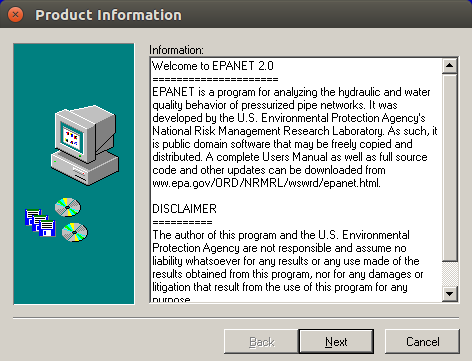
\includegraphics[scale=.3]{imatges/epanet/inst/1.png}
		\end{figure}
		\item Elegir el directori d'instal·lació (típicament C:$\backslash$Program Files)
		\begin{figure}[h!]
			\centering
			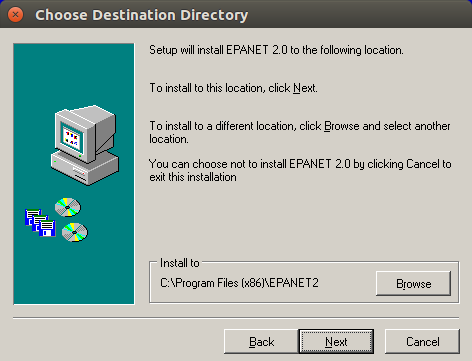
\includegraphics[scale=.3]{imatges/epanet/inst/2.png}
		\end{figure}
		\item Finalitzar l'instal·lació.
		\begin{figure}[h!]
			\centering
			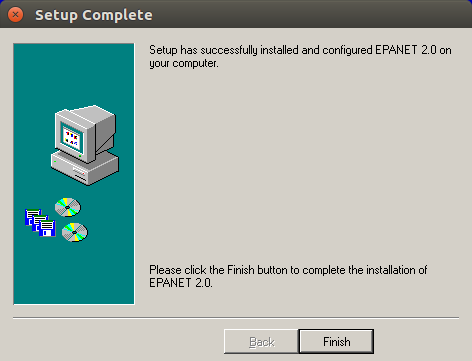
\includegraphics[scale=.3]{imatges/epanet/inst/3.png}
		\end{figure}
		\item Iniciar el programa.
		\begin{figure}[h!]
			\centering
			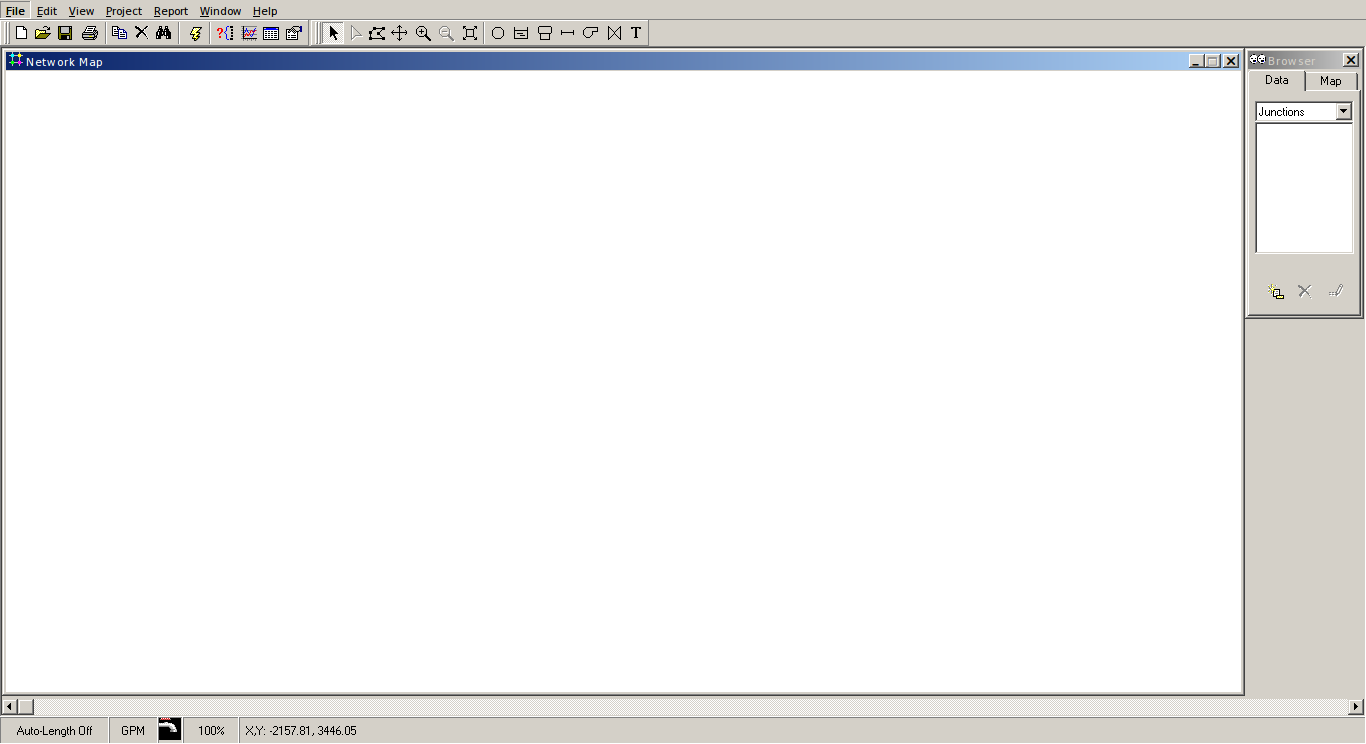
\includegraphics[scale=.15]{imatges/epanet/inst/4.png}
		\end{figure}
	\end{itemize}
\end{itemize}

\subsection{Configuració bàsica de l'entorn}
El primer que cal fer per analitzar una xarxa utilitzant l'eina EPANET és configurar el \textit{layout} del projecte per a que treballi amb les unitats del sistema internacional (litres, metres, segons, etc).
\\\\Per això cal anar a \path{Menu/Projects/Defaults} i en la pestanya \textit{Hydraulics} establir les unitats de fluxe a LPS (Litros por segundo).
\begin{figure}[h!]
	\centering
	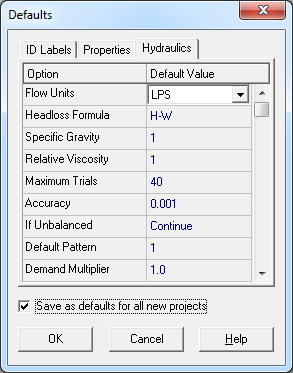
\includegraphics[scale=.7]{imatges/epanet/1.png}
	\caption{Establir les unitats del sistema internacional.}
\end{figure}
\\\\La representació gràfica dels components es pot modificar des de \path{Menu/View/Options}
\begin{figure}[h!]
	\centering
	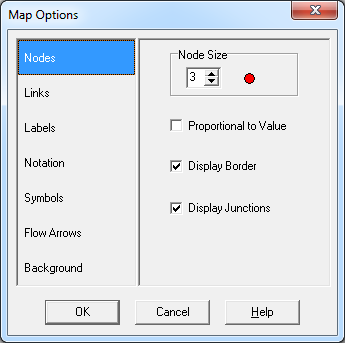
\includegraphics[scale=.7]{imatges/epanet/2.png}
	\caption{Configuració de les propietats dels components gràfics}
\end{figure}
\\\\El límit de coordenades (marge inferior esquerra i el marge superior dret) es pot configurar des del menú \path{Menu/View/Dimensions}
\begin{figure}[h!]
	\centering
	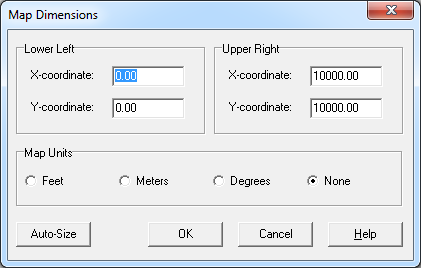
\includegraphics[scale=.7]{imatges/epanet/3.png}
	\caption{Configuració de les dimensions de l'escenari.}
\end{figure}

\pagebreak
\subsection{Implementació d'una nova xarxa de distribució\label{xarxaEPANET}}
En aquest apartat es mostrarà un exemple bàsic de creació d'una xarxa de distribució d'aigua.
\subsubsection{Eines}
Per crear una nova xarxes s'utilitzen els components de la barra d'eines del planol\footnote{Si aquesta barra d'eines no està visible es pot activar des de \path{Menu/View/Toolbars/Map}}.
\begin{figure}[h!]
	\centering
	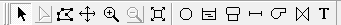
\includegraphics[scale=1]{imatges/epanet/4.png}
	\caption{Eines disponibles per la creació de xarxes.}
\end{figure}
Algunes de les eines més importants són...

\subsubsection{Disseny}
En primer lloc repartim els components que composen la xarxa, en aquest disposem de:
\begin{itemize}
	\item 1 diposit (1)
	\item 8 nodes (2-9)
	\item 1 tanc (10)
\end{itemize}
Aquesta reporesentació quedarà de la següent manera.
\begin{figure}[h!]
	\centering
	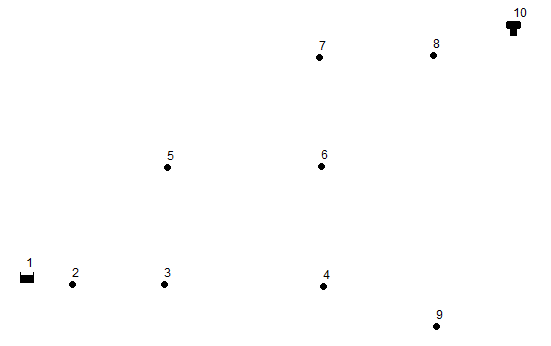
\includegraphics[scale=.7]{imatges/epanet/5.png}
	\caption{Diagrama sense connexions.}
\end{figure}
Ara toca connectar els components a través de tuberies, per això, fem les seguents connexions 1-2, 3-4, 4-9, 3-5, 5-6, 5-7\footnote{Com que aquesta connexió no és recta, cal reseguir el camí per representar la corba de la tuberia.}, 6-7, 4-6. 
\\\\Tot seguit connectem els nodes 2-3 amb una bomba i els nodes 4-9 i 7-8 amb una vàlvula.
\\\\L'estructura de la xarxa hauria de ser similar a la de la següent imatge
\begin{figure}[h!]
	\centering
	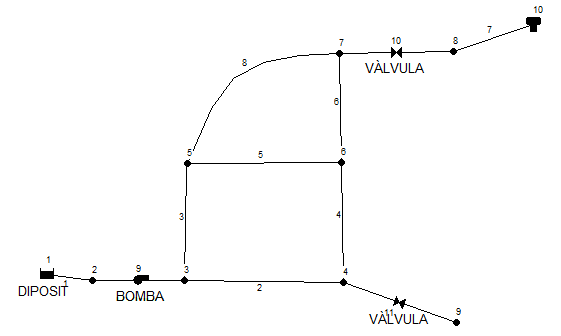
\includegraphics[scale=.7]{imatges/epanet/6.png}
	\caption{Diagrama amb connexions.}
\end{figure}
Un cop es té la distribució dels components, cal assigar les propietats que caracteritzen a cada component, per això s'ha de fer doble clic sobre el component i canviar els seus valors.
\\\\Per aquest exemple canviarem les següents propietats.
Diposit

Tanc

Bomba

Configuració de la corva característica de la bomba, per això seleccionem \say{curve} del desplegable del \say{browser} i creem una nova corba.
\begin{figure}
	\centering
	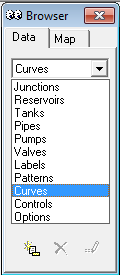
\includegraphics[scale=0.7]{imatges/epanet/10.png}
	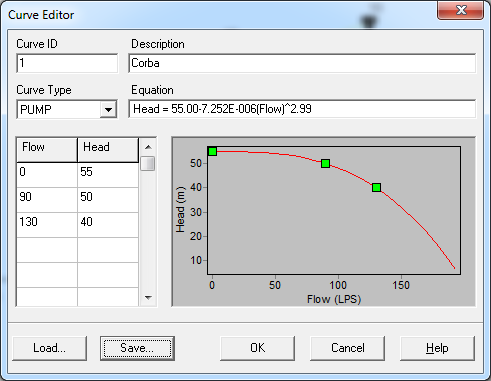
\includegraphics[scale=0.5]{imatges/epanet/11.png}
	\caption{Creació d'una nova corba.}
\end{figure}


\subsection{Anàlisi simple}
Arribats a aquest punt, ja disposem de suficient informació per realitzar un anàlisi hidràulic de regim permanent. El primer que farem és guardar el model\footnote{El format d'emmagatzemament per defecte dels projectes és binari.}, seguidament, per executar el model cal fer clic al botó \path{Menu/Project/Run Analisys}. Si tot ha anat bé hauria de sortir la següent finestre informativa.
\begin{figure}[h!]
	\centering
	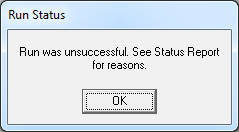
\includegraphics[scale=.5]{imatges/epanet/12.png}
	\caption{Execució correcte.}
\end{figure}
Per veure els resultats de l'execució en format de taula, es pot accedir a través de \path{Menu/Report}, en la seguent taula es pot veure el resultat de l'execució per aquest model.
\begin{figure}[h!]
	\centering
	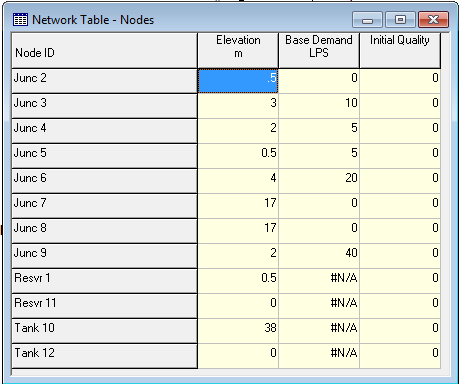
\includegraphics[scale=.5]{imatges/epanet/13.png}
	\caption{Taula de resultats de l'execució.}
\end{figure}

\pagebreak
\subsection{Anàlisi de periòde variant}
Per fer el model més realista, es pot adaptar per a que la demanda dels nodes variï de forma periódicament en funció del temps, això es farà gràcies a un patró que assignarem com a corba de modulació. 
\\\\Per aquest exemple, configurarem la xarxa de tal manera que la \textbf{necessitat dels nodes variï 4 vegades durant el dia} (cada 6 hores) i la \textbf{simulació duri 3 dies} (72 hores). Per a establir aquesta configuració s'ha de seleccionar l'opció \path{Browser/Options/Time} i assignar un valor de 72 a la variable \textit{Total duration} i un valor de 6 a la variable \textit{Pattern time step}.
\begin{figure}[h!]
	\centering
	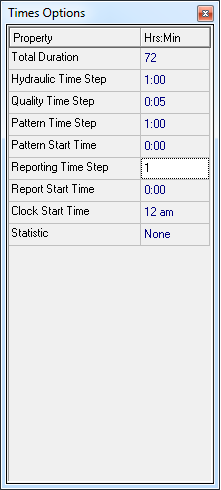
\includegraphics[scale=.7]{imatges/epanet/15.png}
	\caption{Configuració dels intervals de temps.}
\end{figure}
Un cop tenim configurada la freqüència de variació, cal configurar el grau de demanda a cada interval, com que tenim quatre intervals, calen quatre valors que en aquest cas seran [0.5, 1.3, 1.0, 1.2] pels corresponents intervals. Per fer aquesta configuració crearem un patró, i per fer això, anem a \path{Browser/Options} i els valors assignats han de quedar com en la següent imatge.
\begin{figure}
	\centering
	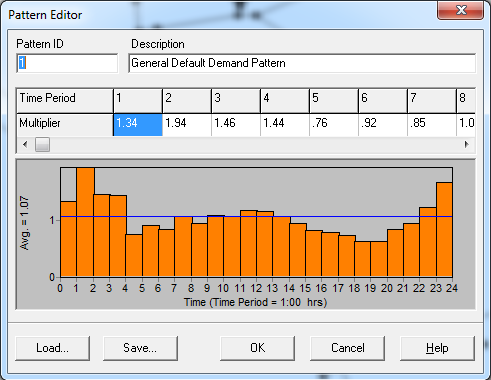
\includegraphics[scale=.5]{imatges/epanet/16.png}
	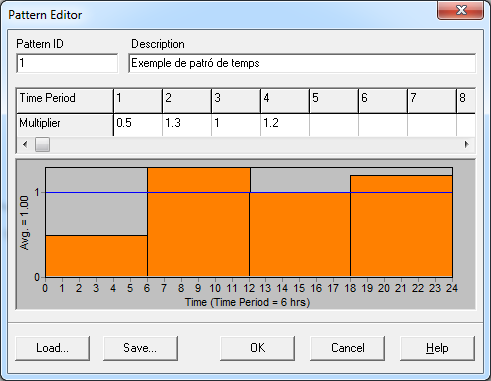
\includegraphics[scale=.7]{imatges/epanet/17.png}
	\caption{Configuració del patró pel temps.}
\end{figure}
Un cop es té creat el patró, s'ha d'assignar com a corba de modulació, per a fer això hi ha dues opcions:
\begin{itemize}
	\item Configurar cada noda amb el patrò (\ref{fig:confNodeAnode}).
	\item Establir una configuració global per tots els nodes (\path{Menu/Porject/Defaults.../Hydraulics}, \ref{fig:confGlobal}).
\end{itemize}
\begin{figure}[h!]
	\centering
	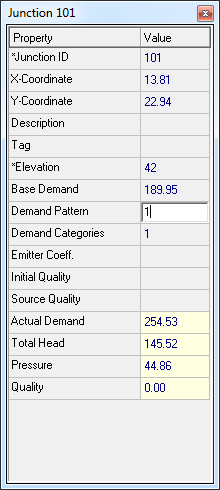
\includegraphics[scale=.7]{imatges/epanet/18.png}
	\label{fig:confNodeAnode}
\end{figure}
\begin{figure}[h!]
	\centering
	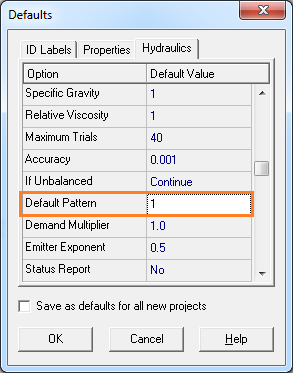
\includegraphics[scale=.7]{imatges/epanet/19.png}
	\label{fig:confGlobal}
\end{figure}
En aquest punt, tornem a executar el model des de 

\subsection{Analisi de la qualitat de l'aigua}
Per veure com es comporta l'aigua a mesura que es distribueix per la xarxa, s'ha implementat una xarxa més sencilla on hi ha un diposit d'on surt l'aigua, ha de passar per un node amb una demanda de 5 LPS i finalment arriba al tanc.

\subsection{Propietats}
En aquest apartat es descriuen algunes de les propietats del programa.

\subsubsection{Algorismes utilitzats en l'anàlisi}
En el manual d'usuari\cite{DocuEpanet} es descriuen detalladament els algorismes utilitzats en el informe de resultats de la qualitat de l'aigua.

\subsubsection{Format dels fitxers}
\textit{Text ASCII}
Els fitxers de tipus text que es poden importar i exportar des de EPANET estan definits per un seguit de capçaleres i les seves propietats, on cada capçalera correspon a un component representable. En la següent imatge es llisten els components disponibles.
\begin{figure}[h!]
	\centering
	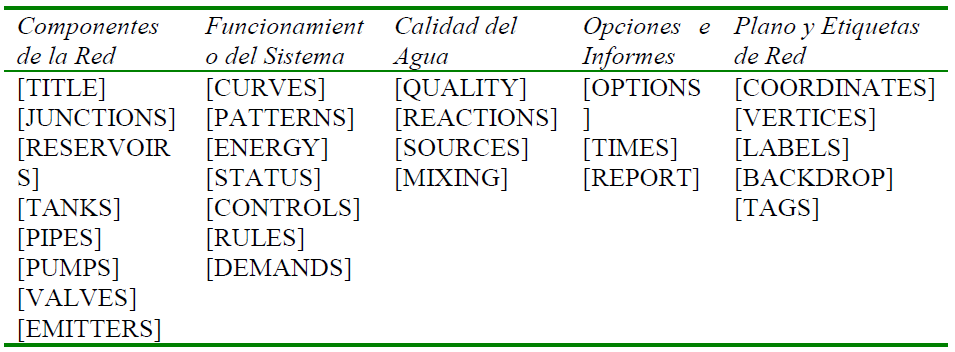
\includegraphics[scale=.5]{imatges/epanet/components.png}
	\caption{Representació dels components d'EPANET}
\end{figure}
Per exemple, per exportar la xarxa desenvolupada en la secció \ref{xarxaEPANET} s'ha d'accedir a \path{Menu/Expor/Map} i seleccionar el format que volem exportar, en aquest cas exportarem la xarxa sencera, i per això, seleccionem \textit{Network...} i li assignem un nom. El contingut del arxiu per aquesta xarxa es pot veure en l'annex \ref{ann1}.

\subsubsection{Interpretació dels errors}
En el moment d'executar la simulacció, es poden produir diversos errors en l'anàlisi, alguns exemples són:
\begin{itemize}
	\item 101: Anàlisi interrumput per falta de memòria.
	\item 110: Anàlisi interrumput degut a que les ecuacions hidràuliques establertes no es poden resoldre.
	\item 202: Valor numèric ilegal assignat a una propietat.
\end{itemize}
El llistat complet dels errors es pot consultar en l'annex B del manual d'usuari\cite{DocuEpanet}.

\clearpage
\subsection{Conclusió d'EPANET}
L'eina EPANET és intuitiva i sencilla d'utilitzar, pot carregar models que estan en diferents formats i de cara al problema plantejat en la secció \ref{problema} pot ser util a l'hora de modelar la xarxa que s'ha d'anal·litzar.

\subsection{Altres exemples}
Alguns exemples de models de xarxes extrets d'Internet.
\begin{figure}[h!]
	\centering
	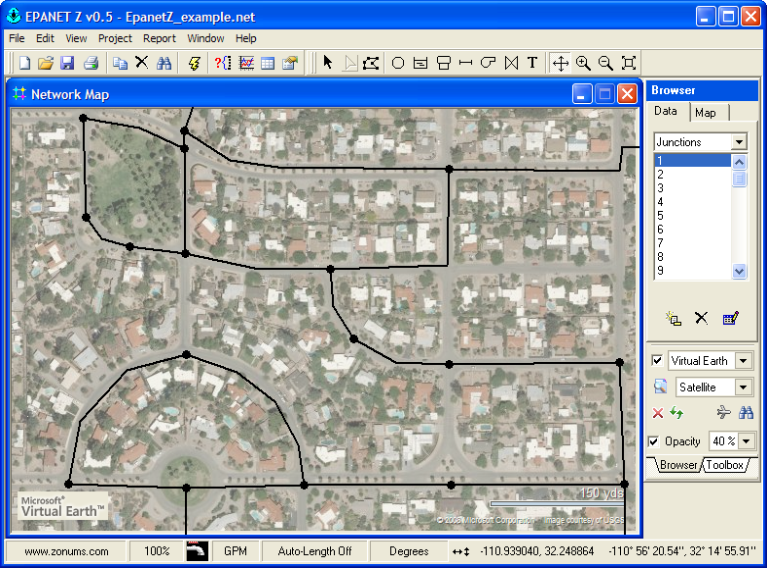
\includegraphics[width=65mm, height=50mm]{imatges/epanet/exemples/x1.png}
	\hspace{.2cm}
	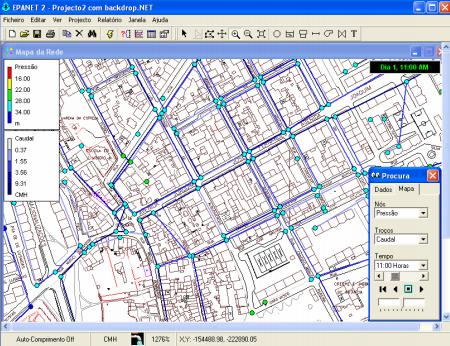
\includegraphics[width=65mm, height=50mm]{imatges/epanet/exemples/x2.jpg}
	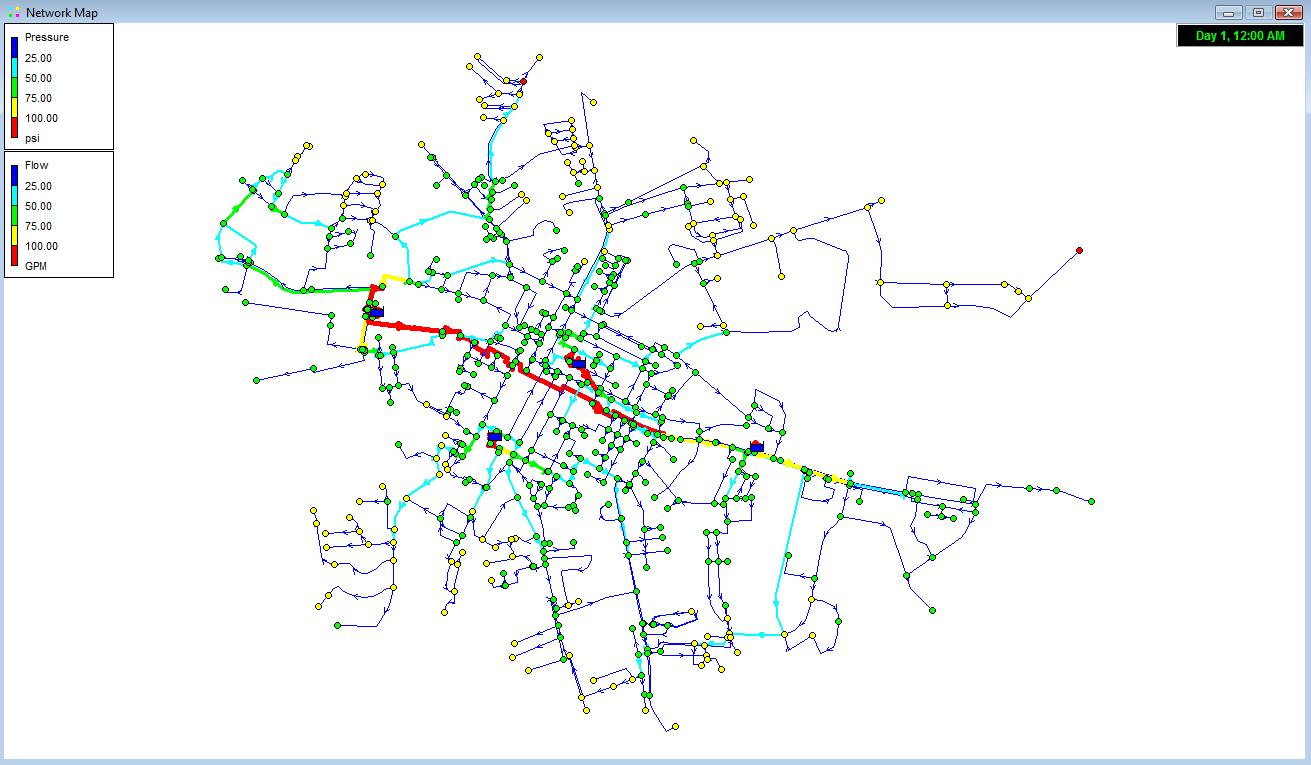
\includegraphics[width=65mm, height=50mm]{imatges/epanet/exemples/x3.jpg}
	\hspace{.2cm}
	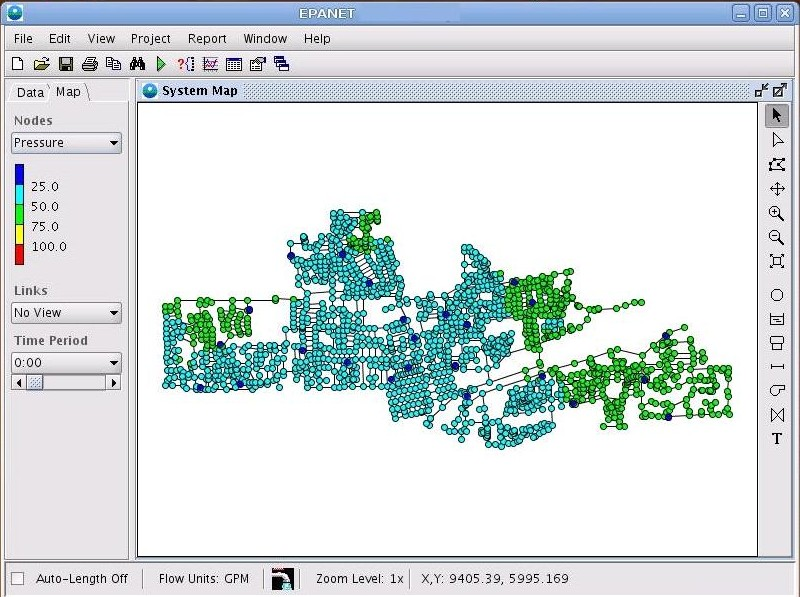
\includegraphics[width=65mm, height=50mm]{imatges/epanet/exemples/x4.jpg}
	\caption{Exemple de xarxes extretes d'Internet}
\end{figure}

%%%%%%%%%%%%%%%TEVA-SPOT%%%%%%%%%%%%%%%%%
\clearpage
\section{TEVA-SPOT Toolkit}
En aquesta secció es mostra com es pot modelar un problema de posicionament de sensors sobre una xarxa de distribució d'aigua, utilitzat l'eina TEVA-SPOT.

\subsection{Instal·lació}
Aquesta eina disposa d'una línea de comandes i d'una interficie gràfica, segons les necessitats de cada usuari es pot utilitzar una versió del programa o una altre.
\subsubsection{Linia de comandes}
Descarregar els binaris del programa \cite{tevaSpotExec}.

\subsubsection{Interfície gràfica}
L'eina TEVA-SPOT Toolkit també disposa d'una interfície gràfica\cite{tevaSpotGui} per facilitar i agilitzar la seva utilització. En aquest document i en la mesura que sigui possible, s'utilitzarà aquesta eina.

\subsubsection{Configuració}

\subsection{Metodologia de posicionament de sensors}
Hi ha diferentes metodologies per resoldre el problema del posicionament de sensors\footnote{Metodologies basades en l'opinió d'experts, mètodes de ranking, optimització, etc.}, la metodologia utilitzada per TEVA-SPOT Toolkit és l'optimització on l'objectiu és trobar una configuració de sensors que minimitzi el risc dels contaminants.

\subsection{Exemple}
Per veure el funcionament d'aquesta eina, s'analitzarà una de les xarxes que ja ve com a exemple amb el programa. Aquesta xarxa és la \textit{Net3} i compta amb 97 nodes.




%%%%%%%%%%%%%%%DOCUMENTACIÓ%%%%%%%%%%%%%%%%%
\clearpage
\section{Documentació utilitzada}
La documentació disponible i que s'ha seguit per elaborar aquest manual és:
\begin{itemize}
	\item Manual d'usuari d'EPANET (\path{/docs/EPANET.pdf)}.
	\item Manual d'usuari del TEVA-SPOT Toolkit (\path{/docs/TEVA-SPOT.pdf}).
	\begin{itemize}
		\item Introducció.
		\item Utilització bàsica.
		\item Formulació a utilitzar per presentar un problema de posicionament de sensors.
		\item Incidents contaminants i impacte de les mesures.
		\item Solvers disponibles.
		\item Format de les dades.
	\end{itemize}
	\item Manual d'usuari per utilitzar la interfície gràfica de TEVA-SPOT Toolkit (\path{/docs/TEVA-SPOT-GUI.pdf}).
\end{itemize}




%%%%%%%%%%%%%%%BIBLIOGRAFIA%%%%%%%%%%%%%%%%%
\clearpage
\begin{thebibliography}{9}
	\bibitem{epanet}\textit{EPANET}:
  	\\\path{https://www.epa.gov/water-research/epanet}
  	
  	\bibitem{DocuEpanet}\textit{Documentació EPANET}:
  	\\\path{http://epanet.info/manuales/}
  	
	\bibitem{tevaSpot}\textit{TEVA-SPOT}:
  	\\\path{https://software.sandia.gov/trac/spot/wiki}

  	\bibitem{tevaSpotExec}\textit{TEVA-SPOT EXECUTABLE}:
  	\\\path{https://software.sandia.gov/trac/spot/downloader}

	\bibitem{tevaSpotGui}\textit{TEVA-SPOT Interfície gràfica}:
  	\\\path{https://cfpub.epa.gov/si/si_public_record_report.cfm?subject=Homeland\%20Security\%20Research&dirEntryId=257684}
\end{thebibliography}

\clearpage
\begin{appendices}
\section{Xarxa 1\label{ann1}}
En aquest annex es mostra el contingut del fitxer per la xarxa desenvolupada en aquest document.\footnote{Aquest mateix fitxer es pot trobar en \path{/xarxes/primera.inp}}
\lstinputlisting[language={}]{xarxes/primera.inp}
\end{appendices}
\end{document}